
\section{Teoría de Funciones}

En esta sección estudiamos uno de los conceptos más relevantes en matemática: el de \textit{función}. De manera intuitiva, este objeto denominado función, corresponde a una \textit{correspondencia o relación} entre elementos de un determinado conjunto con los de otro conjunto. 

Esta noción resulta fundamental para el planteamiento de modelos matemáticos, económicos, físicos y prácticamente para cualquier otra ciencia que utilice matemáticas. 

\subsection{Definiciones preliminares}

\begin{figure}[H]
	\begin{center}
	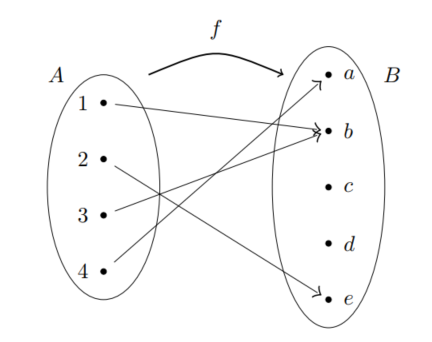
\includegraphics[scale=0.5]{figuras/capitulo1/03-funciones/funcion.png}
		\caption{Función de $A$ en $B$}
		%\label{fig:1_2_inclusion}
	\end{center}
\end{figure}

\begin{definicion}
	\textbf{(Función)}
	Sean $A$ y $B$ dos conjuntos no vacíos de naturaleza arbitraria. Una \textbf{función} $f$ de $A$ en $B$ es una correspondencia entre los elementos de $A$ y los elementos de $B$ de modo tal que a cada $x \in A$ se le hace corresponder un y solo un elemento $y \in B$. Escribimos: 
	\begin{eqnarray*}
		f: A & \longrightarrow & B \\
		x & \longrightarrow & y = f(x) 
	\end{eqnarray*}
	Muchas veces supondremos que $A \subseteq \R$ y que $B = \R$. A estas funciones las llamamos reales de variable real. 
\end{definicion}

\textbf{Notación:} 
\begin{itemize}
	\item Al conjunto $A$ se le llama \textbf{dominio} de $f$. 
	\item Al conjunto $B$ se le llama \textbf{codominio} de $f$. 
	\item Al elemento $y = f(x) \in B$ se le llama \textbf{imagen} de $x$ por $f$. 
\end{itemize}

\begin{definicion}
	\textbf{(Ceros de una función)}
	Sea $f: A \subseteq \R \longrightarrow \R$. Llamaremos \textbf{ceros} de $f$ a todos los reales de su dominio tales que $f(x) = 0$. En estos puntos  el gráfico de $f$ corta al eje OX. 
\end{definicion}

\begin{definicion}
	\textbf{(Conjunto imagen)}
	Sea $f: A \subseteq \R \longrightarrow \R$. Llamaremos \textbf{conjunto imagen} de $f$ al conjunto definido por: 
	$ Im(f) = f(A) = \{ y \in \R: \exists x \in A; y = f(x) \} $ 
\end{definicion}

\begin{definicion}
	\textbf{(Función par)}
	Diremos que $f: A \subseteq \R \longrightarrow \R$ es una \textbf{función par} si y solo si: 
	\begin{itemize} 
		\item $\forall x \in A, -x \in A$. 
		\item $\forall x \in A, f(-x) = f(x)$.
	\end{itemize} 	
\end{definicion}

\begin{definicion}
	Diremos que $f: A \subseteq \R \longrightarrow \R$ es una \textbf{función impar} si y solo si: 
	\begin{itemize}
		\item $\forall x \in A, -x \in A$. 
		\item $\forall x \in A, f(-x) = - f(x)$. 
	\end{itemize} 
\end{definicion}

\begin{ejemplo}
	La función $f(x) = x^2$ es una función par, mientras que la función $g(x) = x^3$ es una función impar. 
\end{ejemplo}

\begin{nota}
	Notar que: 
	\begin{itemize}
		\item El gráfico de una función par es simétrico con respecto al eje $OY$. 
		\item El gráfico de una función impar es simétrico con respecto al origen $O$ del sistema de coordenadas. 
	\end{itemize}
\end{nota}


\begin{definicion}
	\textbf{(Crecimiento de funciones)}
	Sea $f: A \subseteq R \longrightarrow \R$, diremos que: 
	\begin{itemize}
		\item $f$ es \textbf{creciente} en $ A$ ssi $\forall x_1, x_2 \in X$, $x_1 < x_2 \Longrightarrow f(x_1) \leq f(x_2)$. 
		\item $f$ es \textbf{decreciente} en $A$ ssi $\forall x_1, x_2 \in X$, $x_1 < x_2 \Longrightarrow f(x_1) \geq f(x_2)$. 
	\end{itemize} 
	Diremos que el crecimiento o decrecimiento es \textbf{estricto} cuando las desigualdades de las definiciones anteriores se satisfacen de forma estricta. 
\end{definicion}

\begin{definicion}
	\textbf{(Monotonía)}
	Diremos que $f$ es \textbf{monótona} si es creciente o decreciente. 
\end{definicion}

\begin{nota}
	Notar que la negación de la frase $f(x)$ es creciente \underline{no corresponde} a la frase $f(x)$ es decreciente.
\end{nota}

\begin{ejemplo}
	Algunos casos particulares que ejemplifican las definiciones anteriores son: 
	\begin{itemize}
		\item La función $f(x)= -x$ es una función estrictamente decreciente. 
		\item La función $g(x) = x^2$ no es creciente ni decreciente. 
		\item La función $h(x) = 4$ es una función creciente y decreciente a la vez. 
	\end{itemize}
\end{ejemplo}


\begin{definicion}
	\textbf{(Función acotada)} 
	Sea $f: A \subseteq R \longrightarrow \R$, diremos que: 
	\begin{itemize}
		\item $f$ es \textbf{acotada inferiormente} si $\exists a \in \R$ tal que $\forall x \in A, a \leq f(x)$. 
		\item $f$ es \textbf{acotada superiormente} si $\exists b \in \R$ tal que $\forall x \in A, f(x) \leq b$. 
		\item $f$ es \textbf{acotada} si $\exists a, b \in \R$ tales que $\forall x \in A, a \leq f(x) \leq b$. 
	\end{itemize}
\end{definicion}

\begin{proposicion}
	La función $f$ es acotada ssi $\exists M \in \R^+ $ tal que $\forall x \in A, |f(x) | \leq M$. 
\end{proposicion}

\begin{proof}
	\textcolor{red}{To be added..}
\end{proof}

\begin{definicion}
	\textbf{(Máximo y mínimo)}
	Sea $f: A \subseteq R \longrightarrow \R$, diremos que: 
	\begin{itemize}
		\item $x_0 \in A$ es \textbf{punto mínimo} de $f$ si $\forall x \in A, f(x_0 ) \leq f(x)$. Escribimos: $ f(x_0) = \min_{x\in A} f(x)$. 
		\item  $x_0 \in A$ es \textbf{punto máximo} de $f$ si $\forall x \in A, f(x_0 ) \geq f(x)$. Escribimos: $ f(x_0) = \max_{x\in A} f(x)$. 
	\end{itemize}
\end{definicion}

\subsection{Álgebra de funciones}

En el capítulo anterior, sobre conjuntos, estuvimos interesados en la operatoria que podemos realizar entre pares o grupos de conjuntos para definir conjuntos nuevos. A este tipo de operaciones la llamamos \textit{álgebra de conjuntos}. De manera análoga, estudiaremos el \textit{álgebra de funciones} \textcolor{red}{to be fixed...}

\begin{definicion}
	\textbf{(Suma, diferencia, ponderación, producto y cuociente de funciones)}
	Sean $f$ y $g$ dos funciones de dominio $D_f$ y $D_g$ respectivamente y sea $\lambda \in \R$ una constante fija. Definimos las \textbf{funciones suma, diferencia, ponderación, producto y cuociente} por: 
	\begin{itemize}
		\item Suma: $f + g : D_f \cap D_g \longrightarrow \R$ tal que $\forall x \in D_f \cap D_g, (f+g) (x) = f(x) + g(x)$. 
		\item Diferencia: $f - g = f + (-g) $. 
		\item Ponderación: $\lambda f: D_f \longrightarrow \R$ tal que $\forall x \in D_f , (\lambda f)(x) = \lambda f(x)$.
		\item Producto: 
		$ f\cdot g: D_f \cap D_g\longrightarrow \R$ tal que $\forall x \in D_f \cap D_g , (f\cdot g) (x) = f(x) \cdot g(x)$
		\item Cuociente: $\dfrac{f}{g}: A \longrightarrow \R$ tal que $\forall x \in A, \left(\dfrac{f}{g}\right)(x) = \dfrac{f(x)}{g(x)}$, donde $A = D_f \cap D_g \setminus \{ x \in D_g: g(x) = 0\}$ 
	\end{itemize}
\end{definicion}

\begin{definicion}
	\textbf{(Composición de funciones) Sean $A,B,C$ conjuntos y $f: A\rightarrow B$, $g: B\rightarrow C$ funciones. Se define la \textbf{composición} de $f$ y $g$ como la función $g \circ f$ definida por $g \circ f : A \rightarrow C$ tal que $ \forall x \in A, (g \circ f)(x) = g(f(x))$. 
	}
\end{definicion}

\begin{figure}[H]
	\begin{center}
		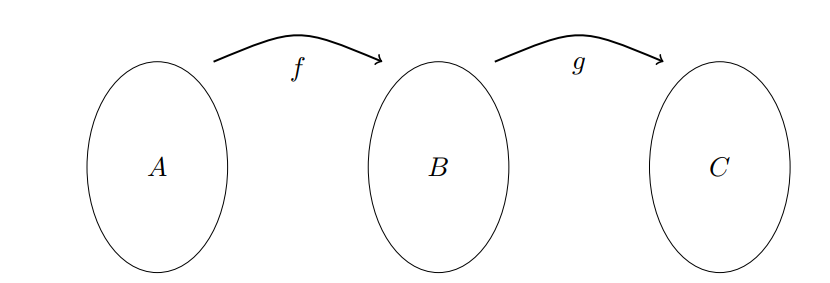
\includegraphics[scale=0.5]{figuras/capitulo1/03-funciones/composicion.png}
		\caption{Composición de funciones}
		%\label{fig:1_2_inclusion}
	\end{center}
\end{figure}

\begin{nota} 
	Notar que no siempre es posible componer funciones. En particular, podría ser que $g \circ f$ quedara bien definida, pero no así $f \circ g$. ¿En qué caso ocurre algo así? 
\end{nota}

\begin{proposicion}
	Sean $f: A \longrightarrow B, g: B \longrightarrow C$ y $h : C \longrightarrow D$ funciones. Se tiene que: 
	\begin{itemize}
		\item $\circ$ es asociativa: $h \circ ( g \circ f) = ( h \circ g ) \circ f $
		\item $id_B$ es neutro por la izquierda para $\circ$ en las funciones de $A$ en $B$: $id_B \circ f = f$ 
		\item $id_A$ es neutro por la derecha para $\circ$ en las funciones de $A$ en $B$: $f \circ id_A = f$. 
	\end{itemize}
\end{proposicion}

\begin{proof}
	\textcolor{red}{To be added..}
\end{proof}

\begin{nota}
	La composición de funciones no es conmutativa. ¿Cuál es un contraejemplo? 
\end{nota}

\begin{definicion}
	\textbf{(Inyectividad)}
	Diremos que una función $f: A \rightarrow B$ es \textbf{inyectiva} si se cumple que: 
	$$ \forall x_1, x_2 \in A , x_1 \neq x_2 \Longrightarrow f(x_1) \neq f(x_2) $$ 
	O, equivalentemente, si se cumple que: 
	$$ \forall x_1, x_2 \in A , f(x_1) = f(x_2) \Longrightarrow x_1 = x_2 $$ 
\end{definicion}

\begin{definicion}
	\textbf{(Sobreyectividad)}
	Diremos que $f: A \rightarrow B$ es \textbf{sobreyectiva} (epiyectiva) si se cumple que: 
	$$ \forall y \in B, \exists x \in A, y = f(x) $$ 
\end{definicion}

\begin{nota}
	 Notar que para que una función \textbf{no} sea biyectiva, basta con encontrar dos elementos distintos de su dominio $x_1$ y $x_2$ tales que $f(x_1) = f(x_2)$.
\end{nota}

\begin{nota}
	Para mostrar que una función \textbf{no} es sobreyectiva, basta encontrar un elemento de su codominio que no pertenezca a su imagen. Es decir, basta encontrar $y$ para el que no exista $x$ en el dominio tal que $f(x) = y$. 
\end{nota}

\begin{definicion}
	\textbf{(Biyectividad)}
	Sea $f: A \rightarrow B$ una función. Diremos que $f$ es \textbf{biyectiva} si es inyectiva y sobreyectiva a la vez. 
\end{definicion}

\begin{proposicion}
	$f: A \rightarrow B$ es biyectiva $\iff \forall y \in B, \exists! x \in A, y = f(x)$
\end{proposicion}

\begin{proof}
	\textcolor{red}{To be added..}
\end{proof}

\begin{definicion}
	\textbf{(Función inversa)}
	Dada $f : A \rightarrow B$ biyectiva, se define la \textbf{función inversa} de $f$, denotada $f^{-1}: B \rightarrow A$, como la función de $B$ en $A$ dada por: 
	$$ \forall x \in A, \forall y \in B, f^{-1}(y) = x \iff y = f(x) $$ 
\end{definicion}

\begin{proposicion}
	Si $f: A \rightarrow B$ es una función biyectiva, entonces su inversa $f^{-1}: B \rightarrow A$ es tal que: 
	\begin{itemize}
		\item $\forall x \in A, f^{-1}(f(x)) = x$. 
		\item $\forall y \in B, f(f^{-1}(y)) = y$. 
	\end{itemize}
\end{proposicion}

\begin{proof}
	\textcolor{red}{To be added..}
\end{proof}

\begin{proposicion}
	Sean $f: A \rightarrow B$ y $g: B \rightarrow C$ funciones. Se tiene que: 
	\begin{itemize}
		\item $f$ y $g$ son inyectivas $\Longrightarrow  g \circ f $ es inyectiva. 
		\item $f$ y $g$ son sobreyectivas $\Longrightarrow  g \circ f $ es sobreyectiva. 
		\item $f$ y $g$ son biyectivas $\Longrightarrow  g \circ f $ es biyectiva. 
		\item $g \circ f$ es inyectiva $\Longrightarrow f$ es inyectiva ($g$ no necesariamente lo es). 
		\item $g \circ f$ es sobreyectiva $\Longrightarrow g$ es sobreyectiva ($f$ no necesariamente lo es). 
	\end{itemize}
\end{proposicion}

\begin{proof}

	Veamos algunas de las demostraciones. 
	
	\begin{itemize}
		\item Supongamos que $f$ y $g$ son sobreyectivas y veamos que $g \circ f$ también lo es.  
		
		Sea $z \in C$. Debemos mostrar que existe $x \in A$ tal que $(g \circ f)(x) = z$, es decir, tal que $g(f(x)) = z$. 
		
		Como $g$ es sobreyectiva, sabemos que existe $y \in B $ tal que $g(y) = z$.  Del mismo modo, como $f: A \rightarrow B$ es sobreyectiva, sabemos que existe $x \in A $ tal que $f(x) = y$. Luego:
		$$ (g \circ f) (x) = g(f(x)) = g(y) = z $$ 
		Se concluye. 
		
		\item Supongamos ahora que $g \circ f$ es inyectiva y veamos que $f$ también lo es. Sean $x_1, x_2 \in A$, tales que: 
		$$ f(x_1) = f(x_2) $$  
		Evaluando en $g$: 
		$$ g(f(x_1)) = g(f(x_2)) $$ 
		Como $g\circ f$ es inyectiva: 
		$$ x_1 = x_2 $$  
		Y se concluye que $f$ es inyectiva. 
		
	\end{itemize}
\end{proof}

\begin{corolario}
	Si $f: A \rightarrow B$ es biyectiva, entonces $f^{-1}$ es biyectiva y $(f^{-1})^{-1} = f$. 
\end{corolario}

\begin{proposicion}
	Si $f: A \rightarrow B$ y $g: B \rightarrow C$ son biyectivas, entonces: 
	$$ (g\circ f)^{-1} = f^{-1} \circ g^{-1} $$ 
\end{proposicion}

\begin{proof}
	Denotemos $F = g\circ f $ y $G = f^{-1}\circ g^{-1}$. Nos basta verificar que: 
	$$ G \circ F = id_A , \quad F \circ G = id_C $$ 
	En efecto: 
	\begin{eqnarray*}
		G \circ F  &=& (f^{-1} \circ g^{-1} ) \circ (g \circ f) \\ 
		&=& f^{-1} \circ ((g^{-1} \circ g) \circ f) \\ 
		&=& f^{-1} \circ (id_B \circ f) \\ 
		&=& f^{-1} \circ f \\ 
		&=& id_A
	\end{eqnarray*}  
	La otra igualdad es análoga. 
\end{proof}

Algunos ejercicios sugeridos para interiorizar los conceptos anteriores se presentan a continuación: 

\begin{ejercicio}
	Estudie la inyectividad, sobreyectividad y biyectividad de la siguiente función. 
	\begin{eqnarray*}
		f: \R^2 &\longrightarrow &\R \\
		(x, y)  &\longrightarrow & x + y
	\end{eqnarray*}
\end{ejercicio}

\begin{ejercicio}
	Considere la función definida por: 
	$$ f(x) = \dfrac{x^2 + 2x - 3}{x^2-1} $$ 
	\begin{enumerate}
		\item Determine: $Dom(f)$ y ceros de $f$. 
		\item Demuestre que $f$ es monótona en $Dom(f) \cap (-1, \infty)$ y en $Dom(f) \cap (-\infty, -1)$.
	\end{enumerate}
\end{ejercicio}


\begin{ejercicio}
	Sea $f: A \subseteq \R \rightarrow \R$ una función par. Demuestre que si $f$ es creciente en $A \cap \R^+$, entonces $f$ es decreciente en $A\cap \R^-$. 
\end{ejercicio}

\begin{ejercicio}
	Sea $f: A \subseteq \R \rightarrow \R$  definida por $f(x) = \dfrac{2 - |x|}{x^2 - 4} $. 
	Se pide determinar dominio de $f$, ceros, paridad y crecimiento.
\end{ejercicio}

\subsection{Referencias}

Apunte Introducción al Álgebra, semanas 4 y 5; Apunte Introducción al Cálculo, semana 5. 